Å skulle diskretisere kvadratet er ikke like trivielt som sirkelen eller ellipsen.
Vi ønsker å skulle kunne gjenbruke samme klasse for integrallikningen, så en polar implementering av diskretiseringen er mest opplagt.
En kontinuerlig mulighet er en såkalt superellipse, som kan diskretiseres med
\[
    \xtt(\theta) = \left( {\absl{\cos{\theta}}}^{\sfrac{2}{N}}\sgn{(\cos{\theta})}, {\absl{\sin{\theta}}}^{\sfrac{2}{N}}\sgn{(\sin{\theta})} \right),
\]
som vil konvergere raskt mot et kvadrat når $N$ blir stor.
Problemet her er at $\theta$ ikke faktisk er vinkelen i parametriseringen.
Parametriseringsvariablen vil bruke lang tid i hjørnene på superellipsen, og en enorm andel av normalvektorene langs randa vil derfor være fullstendig feil.

En enklere løsning vil være å heller kjøre $\theta$ gjennom \texttt{if}-sjekker, som følger.
\begin{algorithm}[H]
    \caption{Konstruer kvadrat}\label{alg:kvadrat}
    \begin{algorithmic}
        \For{$n \leq \mathtt{N}$}
            \If{$\theta_n \in [-\sfrac{\pi}{4}, \sfrac{\pi}{4})$}
                \State $\xtt_n, \ytt_n \gets 2a, 2a\tan{(\theta_n)}$
            \ElsIf{$\theta_n \in [\sfrac{\pi}{4}, \sfrac{3\pi}{4})$}
                \State $\xtt_n, \ytt_n \gets 2a\sec{(\theta)}, 2a$
            \ElsIf{$\theta_n \in [3\sfrac{\pi}{4}, \sfrac{5\pi}{4})$}
                \State $\xtt_n, \ytt_n \gets -2a, -2a\tan{(\theta_n)}$
            \ElsIf{$\theta_n \in [\sfrac{5\pi}{4}, \sfrac{7\pi}{4})$}
                \State $\xtt_n, \ytt_n \gets -2a\sec{(\theta)}, -2a$
            \EndIf
        \EndFor
    \end{algorithmic}
\end{algorithm}

\noindent Denne løsningen er ikke veldig vakker, men den forsikrer at alle nodene faktisk ligger på kvadratet.
Dette kan ikke sies for hjørnene i $\textit{\texttt{ж}}$, ettersom hjørnenodene kan havne innenfor randa i dersom ikke enten $\xtt_p$ eller $\xtt_m$ ligger akkurat i hjørnet for denne $N$-verdien.
Vi ser i figur \ref{fig:added_mass_square_N1000} at dette kan føre til merkelige mønstre i konvergensen til den adderte massen, hvor tilnærmingen faktisk kan bli dårligere for en større $N$-verdi.
\begin{Figure}
    \centering
    \captionsetup{type = figure}
    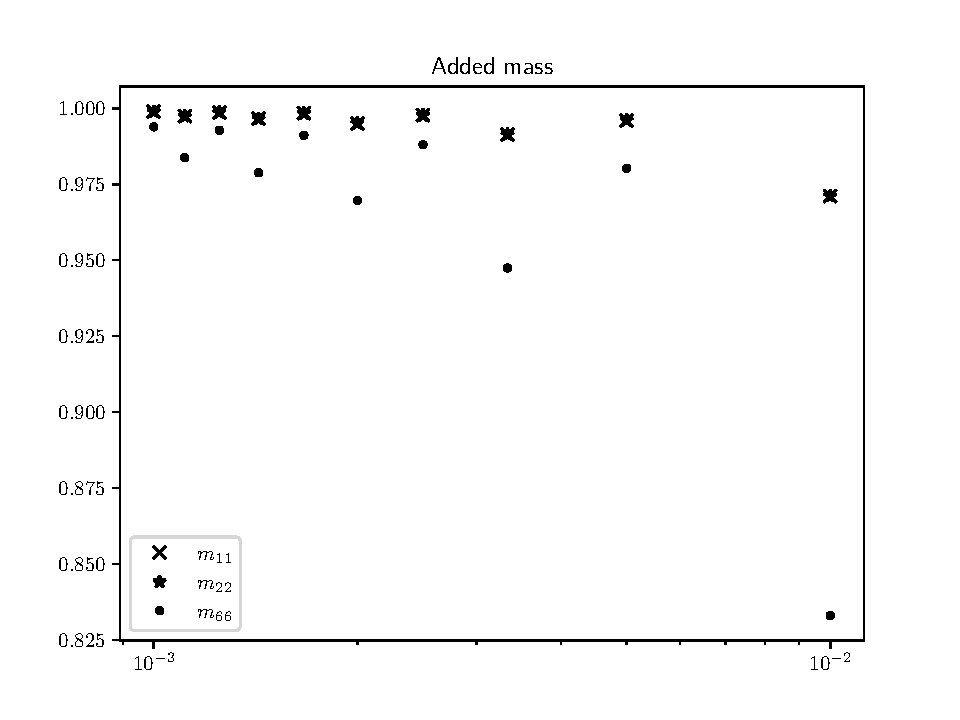
\includegraphics[width = \linewidth]{addedmass_square_N1000.pdf}
    \captionof{figure}{Numerisk utregnet over teoretisk addert masse på et kvadrat.}
    \label{fig:added_mass_square_N1000}
\end{Figure}

\noindent Samtidig ser vi at den utregnede adderte massen fakitsk konvergerer.
Vil man unngå å se denne unøyaktigheten, kan man forsikre seg at $\{ \sfrac{\pi}{4}, \sfrac{3\pi}{4}, \sfrac{5\pi}{4}, \sfrac{7\pi}{4} \} \in \theta$ ved å la $N$ alltid være delelig på 8, slik som i figur \ref{fig:added_mass_square_N640}.
\begin{Figure}
    \centering
    \captionsetup{type = figure}
    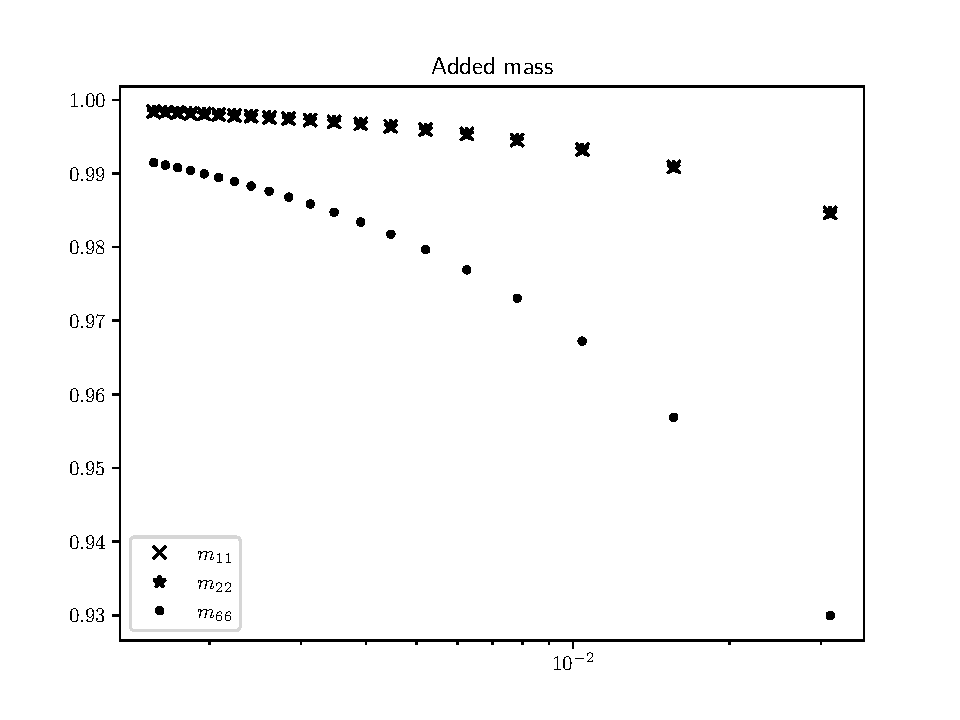
\includegraphics[width = \linewidth]{addedmass_square_N640.pdf}
    \captionof{figure}{Numerisk utregnet over teoretisk addert masse på et kvadrat med $N$ delelig på 8.}
    \label{fig:added_mass_square_N640}
\end{Figure}
\begin{Figure}
    \centering
    \captionsetup{type = figure}
    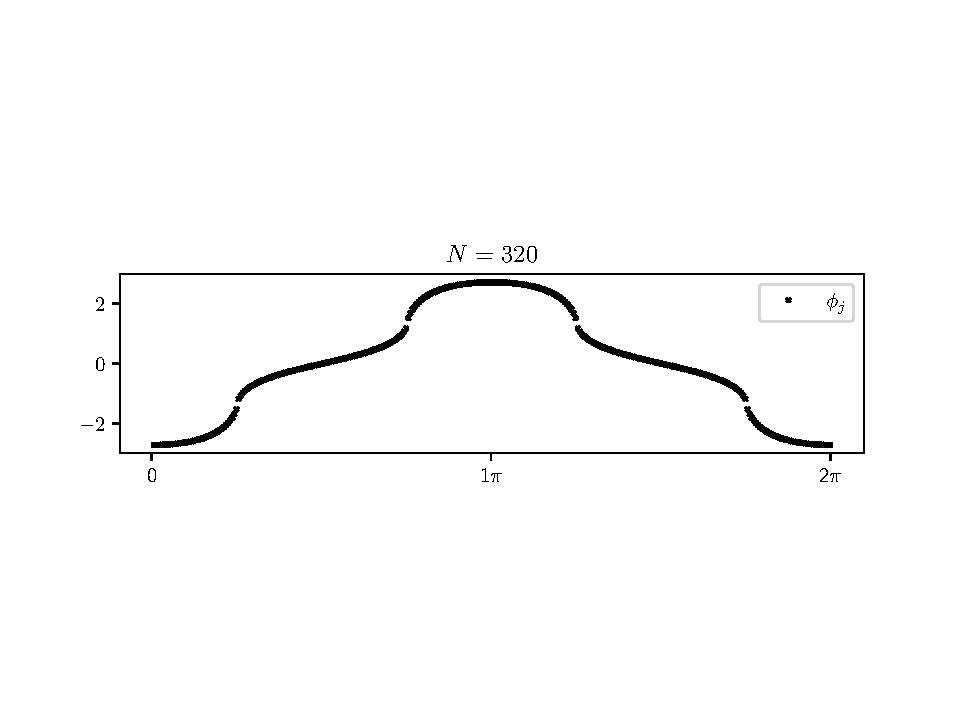
\includegraphics[width = \textwidth]{phi1_N320.pdf}
    \captionof{figure}{$\phi_1$ er gitt numerisk med punkter.}
    \label{fig:phi1_square_N320}
\end{Figure}
\begin{Figure}
    \centering
    \captionsetup{type = figure}
    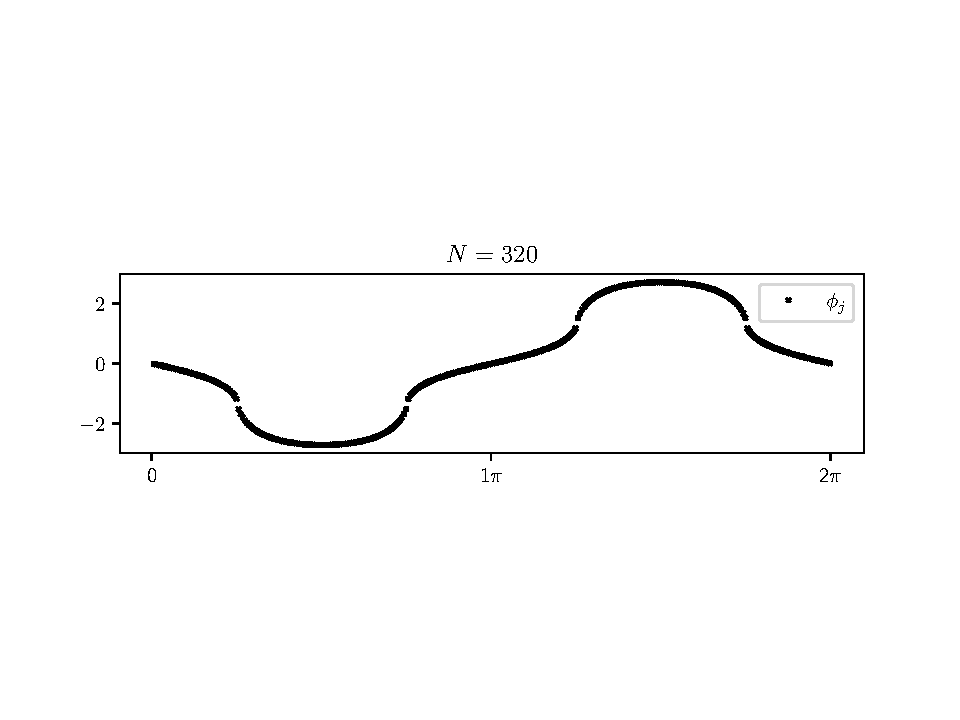
\includegraphics[width = \textwidth]{phi2_N320.pdf}
    \captionof{figure}{$\phi_2$ er gitt numerisk med punkter.}
    \label{fig:phi2_square_N320}
\end{Figure}
\begin{Figure}
    \centering
    \captionsetup{type = figure}
    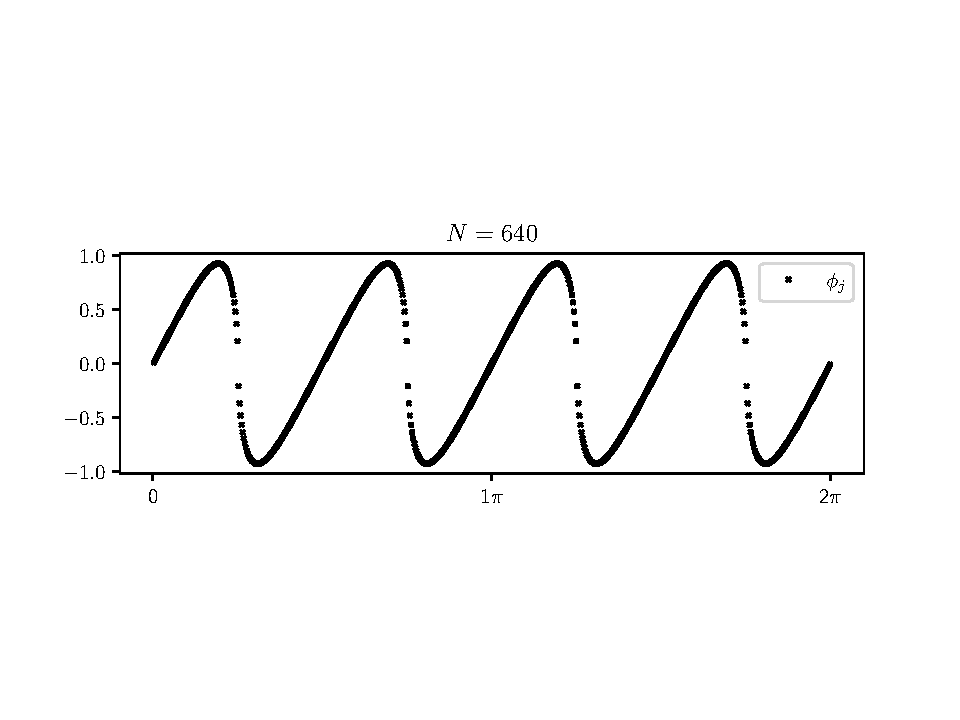
\includegraphics[width = \textwidth]{phi6_N640.pdf}
    \captionof{figure}{$\phi_6$ er gitt numerisk med punkter.}
    \label{fig:phi1_square_N6400}
\end{Figure}